\documentclass[10pt]{article}
\usepackage[utf8]{inputenc}
\usepackage[T1]{fontenc}
\usepackage{amsmath}
\usepackage{amsfonts}
\usepackage{amssymb}
\usepackage[version=4]{mhchem}
\usepackage{stmaryrd}
\usepackage{graphicx}
\usepackage[export]{adjustbox}
\graphicspath{ {./images/} }

\title{CONTROL ROBUSTO DE UN LOOPER DE MOLINO DE BANDAS EN CALIENTE }


\author{Centro de Control Industrial\\
Universidad de Strathclyde.\\
Edificio Graham Hills\\
50 George St. Glasgow G1 1QE,U.K\\
email:gerald@icu.strath.ac.uk}
\date{}


\begin{document}
\maketitle


\begin{abstract}
Se presenta un controlador multivariable para el looper de un molino de bandas en caliente para controlar la tensión y el flujo másico de la banda. El looper es un brazo que empuja contra la tira entre los soportes en un molino en tándem para mantener constante la tensión de la tira y aislar las interacciones de los soportes adyacentes. El controlador está diseñado usando Hinfinity para desacoplar la tensión y el ángulo y también para inferir la tensión no medida. El rendimiento y la robustez de este diseño se demuestran mediante una simulación no lineal de un molino de bandas en caliente.
\fin{resumen}

Palabras clave. Optimización H-infinity, Industria siderúrgica, Inferencia, Control robusto

\section{INTRODUCCIÓN}
En un molino de acabado de bandas en caliente, un looper es un brazo ubicado entre soportes adyacentes, que es accionado por un motor eléctrico o cilindro hidráulico. Las funciones del looper son mantenerse en contacto con la tira para proporcionar una tensión constante de la tira y aislar el funcionamiento de los soportes absorbiendo cualquier error de flujo másico. El looper funciona como un actuador y un sensor, ya que aplica una fuerza a la tira y su ángulo es una medida del flujo másico de la tira. Mantener la banda bajo tensión constante ayuda a mantener la precisión dimensional del calibre de la banda, el ancho y la corona, especialmente cuando los aceros de mayor calidad se laminan a altas velocidades. El control del flujo másico mediante la regulación del ángulo del lazo evita la formación de adoquines peligrosos en la tira y desacopla el control del medidor de cada soporte entre sí.

Un problema importante es controlar la tensión y el ángulo del looper simultáneamente que interactúan entre sí. En la práctica convencional, el looper se controla mediante el uso de dos bucles separados. La tensión se controla indirectamente controlando la corriente del motor looper y el ángulo del looper se controla variando la velocidad del motor de accionamiento principal aguas arriba. Usando este enfoque, el control de la tensión y el ángulo no están suficientemente desacoplados. Aunque el control multivariable de loopers no es común, se han implementado controladores multivariables óptimos en la industria. (Seki et al., 1991; Kishimoto, $1981)$

En este trabajo se presentará el modelado del looper, la tensión de la tira y el flujo másico. La técnica de diseño H-infinity se utilizará para diseñar un controlador para dos casos diferentes. El primer diseño cuando es posible medir la tensión directamente. En el entorno de un molino de bandas en caliente, es costoso y difícil medir la tensión, por lo que se presenta una segunda solución al problema de control donde la tensión se infiere con fines de control. El rendimiento y la robustez de los dos diseños se muestran mediante el uso de una simulación no lineal de un molino de bandas en caliente.

El documento está organizado de la siguiente manera. El modelado de looper se describe en la sección 2. El problema de control se formula en la sección 3. Los resultados de la simulación se presentan en la sección 4, finalmente las conclusiones se extraen en la sección $5 .$

\section{MODELADO DEL SISTEMA}
La Figura 1 muestra un par $T_{m}$ que se aplica al brazo del looper en un ángulo $\theta$ con la velocidad del soporte $\mathrm{i}$ rollos de trabajo siendo $\omega^{i}$, poniendo así la tira bajo una tensión de tracción de $\sigma$.

\begin{center}
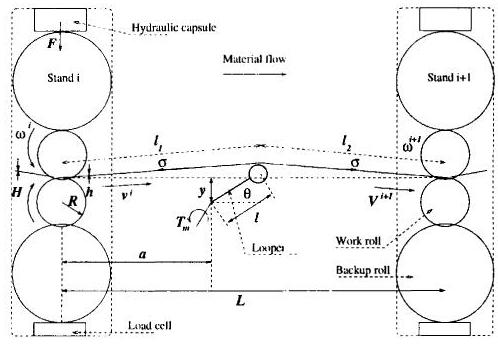
\includegraphics[max width=\textwidth]{2022_06_24_9b97a76a6ff0403ae6ddg-2}
\end{center}

Figura 1. Geometría de looper e interstand

\section{$2.1$ Tensión de tira}
El modelo de tensión se basa en la tensión longitudinal y la deformación definida por el módulo de Young.

$$
\begin{gathered}
\sigma(t)=E\left[\frac{L(\theta(t))-L_{s}(t)}{L_{s}(t)}\right] \\
{\left[(r-y+l \sin \theta)^{2}+(a+l \cos \theta)^{2}\right]^{1 / 2}} \\
{\left[(r-y+l \sin \theta)^{2}+(1-a-l \cos \theta)^{2}\right]^{1}} \\
L_{s}=L_{o}+\int_{t_{0}}\left(v^{i}(\tau)-V^{i+1}(\tau)\right) d \tau
\end{gathered}
$$

$$
\begin{aligned}
& l_{2}=\left[(r-y+l \sin \theta)^{2}+(1-a-l \cos \theta)^{2}\right]^{1 / 2}
\end{aligned}
$$

La deformación depende de la cantidad de material en la región interstand, que depende de la diferencia de velocidad de la tira que sale del stand $i$ y entra en el stand $i+1$. La extensión es la diferencia entre la longitud de la tira geométrica y la longitud de la tira en el interstand. Este análisis asume la geometría de la línea recta para la tira (para efectos catenarios, Grimble 1976).

\section{$2.2$ Mecánica de loopers}
Si el looper tiene una inercia $J_{L}$ con respecto a su pivote, entonces se puede aplicar la segunda ley de Newton.

$$
J_{L} \ddot{\theta}=T_{m}-T_{\text {load }}
$$

donde $T_{\text {load }}$ es el par de carga:

$$
T_{\text {load }}=T_{\sigma}+T_{s}+T_{L W}+T_{b}+T_{d}
$$

El par de carga debido a la tensión de la tira es:

$$
T_{\sigma}=\sigma w h\left[l \cos \theta f_{1}(\theta)+(l \sin \theta+r) f_{2}(\theta)\right]
$$

Dónde

$$
\begin{array}{ll}
f_{1}(\theta)=(r+l \sin \theta-y)\left(\frac{1}{l_{1}}+\frac{1}{l_{2}}\right) \\
f_{2}(\theta)=\left(\frac{L-a-l \cos \theta}{l_{2}}-\frac{a+l \cos \theta}{l_{1}}\right)
\end{array}
$$

El par para soportar el peso de la tira es:

$$
T_{s}=l g \rho w h\left(l_{1}+l_{2}\right) \cos \theta
$$

El par requerido para soportar el brazo del looper y el peso del rodillo es:

$$
T_{L W}=l g M_{r} \cos \theta+\frac{l}{2} g M_{a} \cos \theta
$$

El par requerido para doblar la tira sobre el rodillo del looper es:

$$
T_{b}=l \cos \theta \frac{\sigma_{y s} w h^{2}}{4}\left(\frac{1}{l_{1}}+\frac{1}{l_{2}}\right)
$$

El par de amortiguación por fricción es

$$
T_{d}=r \dot{\theta}
$$

La respuesta del accionamiento que suministra el par al brazo del looper se modela mediante un retraso de primer orden.

\section{$2.3$ Flujo másico}
Desde la entrada hasta la salida del stand, el flujo másico se conserva $(V H=v h)$ suponiendo que el ancho permanezca constante. Entre los rollos de trabajo y la tira, se produce un deslizamiento que es muy sensible a la tensión de la tira. La velocidad de la tira que sale del soporte $\mathrm{i}$ está relacionada con la velocidad de la rueda de trabajo por el deslizamiento hacia adelante $(f)$ :

$$
v^{i}=\left(1+f^{i}\right) \omega^{i} R
$$

El accionamiento principal se modela como un sistema de una masa con un bucle de velocidad local utilizando un controlador PI y un par de carga que es una función de la tensión y la velocidad.

Para el diseño del controlador, el modelo no lineal se linealizó sobre la tensión de operación y el ángulo nominal de $ 15 \mathrm{de}-$ grees. Dado que la tensión depende de la diferencia de velocidad relativa entre los soportes $\mathrm{i}$ y $\mathrm{i}+1$, entonces la velocidad de balanceo del soporte i+1 puede mantenerse constante sin afectar el diseño, aunque la velocidad de la tira que entra en el stand $i+1$ aún puede cambiar debido a la tensión. La Figura 2 muestra la estructura del modelo lineal donde todas las variables son pequeños cambios desde el punto de operación.

\begin{center}
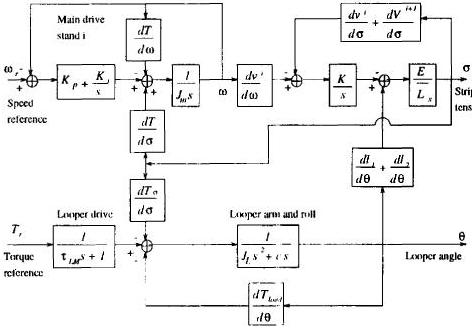
\includegraphics[max width=\textwidth]{2022_06_24_9b97a76a6ff0403ae6ddg-3}
\end{center}

Figura 2. Modelo de sistema linealizado

\section{3. $H_{\infty}$ CONTROI, DISEÑO}
\subsección{Formulación del problema}
El espacio de Hardy $H_{\infty}$ consiste en todas las matrices de función de transferencia propias estables. Si $G(s)$ es una matriz de función de transferencia estable, entonces la norma $H_{\infty}$ se define como:

$$
\| G(s)\|_{\infty}=\sup _{\omega} \sigma[G(j \omega)]
$$

donde $\bar{\sigma}^{2}$ es el valor propio máximo de $\bar{G}^{T} G$. La formulación estándar de dos puertos para el diseño de $H_{\infty}$ se muestra en la figura 3, donde el $P generalizado de la planta contiene la dinámica de la planta aumentada con las funciones de ponderación que especifican el rendimiento deseado del circuito cerrado. La matriz $P(s)$ se divide para tener dos conjuntos de entradas y salidas. El vector $w$ consiste en entradas externas como referencias y perturbaciones, $z$ consiste en señales de error, $y$ son variables medidas y $u$ es la entrada de control. Si la función de transferencia de bucle cerrado de $w$ a $z$ es $T_{z w}$, entonces el problema de diseño estándar es minimizar la norma $H_{\infty}$ de $T_{z w}$ encontrando un controlador $K$ tal que $T_{z w}$ sea internamente estable. La función de transferencia de bucle cerrado viene dada por:

$$
T_{z w}=P_{11}+P_{12} K\left(I-P_{22} K\right)^{-1} P_{21}
$$

El controlador óptimo se encuentra encontrando $\left\| T_{z w}\right\|_{\infty} \leq \gamma$ para todos los controladores $\mathrm{K}$ que estabilizan el bucle cerrado y luego disminuyen $\gamma$ hasta que no se puede encontrar ningún controlador estabilizador. Este problema de optimización para encontrar $K$ se resuelve a través de los resultados de Doyle et al., (1989) y los algoritmos implementados en un paquete de diseño de Matlab (Balas, 1993).

\begin{center}
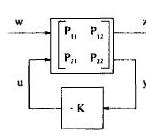
\includegraphics[max width=\textwidth]{2022_06_24_9b97a76a6ff0403ae6ddg-3(1)}
\end{center}

\begin{center}
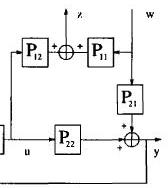
\includegraphics[max width=\textwidth]{2022_06_24_9b97a76a6ff0403ae6ddg-3(2)}
\end{center}

a) Formulario de dos puertos

b) Forma clásica

Figura 3. Configuración estándar

\section{$3.2$ Diseño $I$}
En el diseño I se supone que tanto la tensión como el ángulo se miden. Se introducen ponderaciones en la señal de error y en la señal de control. La configuración del diseño se muestra en la figura 4, donde la planta se aumenta con las dos ponderaciones y filtros para generar señales de referencia y perturbaciones. Las entradas exógenas se generan al pasar ruido blanco a través de los pesos estables $W_{r e f}$ y $W_{\text {dist }}$. Los pesos de rendimiento se eligieron inicialmente para representar el inverso del rendimiento de bucle cerrado deseado y se ajustaron para proporcionar:

$$
W_{1}=\left[\frac{s+6.52}{1.55 s+0.0076}\right], W_{2}=\left[\frac{s+286}{20 s+200000}\right]
$$

Para ambos pesos, todos los elementos de la diagonal inicial son idénticos. Esto podría hacerse porque las salidas de la planta se escalaron especialmente para ponderar más el error de tensión, ya que esto afecta directamente la calidad de la tira, mientras que el ángulo del looper no lo hace. Los valores singulares máximos para las funciones de transferencia de bucle cerrado obtenidas se muestran en la figura 6. El ancho de banda de bucle cerrado es de alrededor

\begin{center}
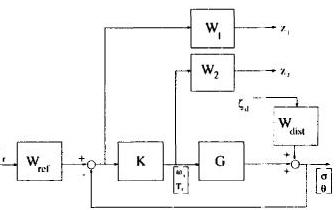
\includegraphics[max width=\textwidth]{2022_06_24_9b97a76a6ff0403ae6ddg-4}
\end{center}

Figura 4. Diseño I aumentado syst.em

$10 \mathrm{rad} / \mathrm{s}$ y tanto el control como la sensibilidad complementaria se despliegan a altas frecuencias. Dado que el inverso de los pesos limita las sensibilidades, el diseño ha alcanzado un rendimiento nominal.

\section{$3.3$ Diseño II}
Para soportar el ambiente hostil en un molino de bandas en caliente donde la temperatura de la banda puede ser de $ 1000^{\circ} \mathrm{C}$ se requiere instrumentación de muy alta calidad. Para medir la tensión directamente se requerirían células de carga en el rodillo del looper, lo que aumenta el gasto y la inercia del looper, disminuyendo así el rendimiento. El control convencional del looper sin una medición de tensión generalmente controlaría indirectamente la tensión variando el par aplicado al looper y su posición se regularía ajustando la velocidad del stand. En este segundo diseño, la medición de tensión no está presente y se elige la medición de la velocidad del soporte para reemplazarla. Usar la velocidad real como entrada al controlador es útil porque la velocidad determina la longitud de la tira en el interstand y la tensión produce un par de carga en el soporte que cambia la velocidad. El sistema aumentado para el diseño inferencial se muestra en la figura 5 con ponderaciones en la señal de control y señales de error. Nuevamente los filtros se colocan en las entradas exógenas. Las ponderaciones diagonales elegidas son:

$$
W_{1}=\left[\frac{s+13.24}{1.73 s+0.0012}\right], W_{2}=\left[\frac{s+266}{0.35 s+13400}\right]
$$

La figura 7 muestra las respuestas de frecuencia de bucle cerrado ob-

\begin{center}
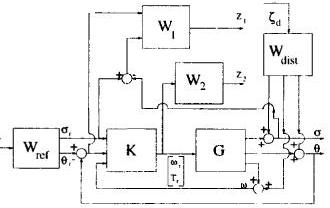
\includegraphics[max width=\textwidth]{2022_06_24_9b97a76a6ff0403ae6ddg-4(1)}
\end{center}

Figura 5. Diseño II, sistema aumentado retenido. El ancho de banda es similar al diseño I, pero la magnitud de la sensibilidad de control es menor y, de nuevo, las sensibilidades están limitadas.

\section{RESULTADOS DE SIMULACIÓN}
Para probar los dos controladores se utiliza una simulación no lineal de un molino caliente de siete soportes. Los loopers se accionan eléctricamente y los resultados mostrados son para el looper situado entre los stands 1 y 2. Se realizaron dos pruebas en cada uno de los diseños; La primera fue cambiar la tensión y el ángulo de referencia y la segunda prueba más importante fue rechazar las perturbaciones de velocidad en el stand 1.

Las figuras 8 y 10 muestran cambios en las referencias para el diseño I y el diseño II, respectivamente. Cambiando la referencia de tensión, el diseño I tiene una respuesta más rápida que el diseño II. Cuando se cambia la referencia del ángulo, el diseño I tiene menos interacción con la tensión que el diseño II. Las tareas principales son regular la tensión y el flujo másico rechazando perturbaciones tales como cambios en el calibre de banda y la temperatura que afectan el par de carga experimentado por los motores de soporte. Las figuras 9 y 11 muestran el efecto de una perturbación de la cápsula de $5 \%$ en el stand 1 (medidor de salida de $14 \mathrm{~mm}$ ), la velocidad del stand se ralentiza aumentando la tensión de la tira. Es más importante regular la tensión de la tira que el ángulo, ya que la tensión afecta directamente a las propiedades dimensionales de la tira. El diseño I limita la magnitud del aumento de tensión de manera efectiva y recupera su tensión de referencia en un tiempo aceptable. Para el diseño II, la magnitud de la tensión aumenta tal vez mayor, pero es el tiempo que la tira pasa en esta tensión lo que hace que el rendimiento sea indeseable.

Como era de esperar, el rendimiento del diseño inferencial en la simulación no lineal no es tan bueno como cuando la medición de tensión está directamente disponible. Este hecho no es tan obvio a partir de los gráficos de bucle cerrado de valor max-singular, ya que ambos diseños tienen aproximadamente el mismo ancho de banda y la sensibilidad del diseño II muestra un mejor rendimiento de seguimiento. Dado que los controladores fueron diseñados para un punto de operación, los resultados de la simulación no lineal muestran la robustez del sistema de control a los efectos no lineales modelados en la simulación.

\section{CONCLUSIÓN}
Se desarrollaron dos estrategias de diseño para controlar un looper de molino de bandas en caliente utilizando la optimización de $H_{\infty}$. Los controladores fueron diseñados con y sin la medición de tensión disponible. Usando una simulación no lineal de un molino de bandas en caliente de siete rodales, se probó el rendimiento de cada diseño y se encontró que cuando se dedujo la tensión de la banda, las cualidades de rechazo de perturbación del looper disminuyeron. Dado que la medición de la tensión en un molino de bandas en caliente es costosa, entonces el rendimiento reducido producido sin medir la tensión puede justificarse en el costo. Se mostraron los resultados para un solo looper, pero dado que las perturbaciones del flujo másico afectan a todos los loopers, entonces un diseño futuro que use $H_{\infty}$ para loopers debe reflejar el control global del flujo másico.

\section{REFERENCIAS}
Balas, G. J., J. C. Doyle, K. Glover, A. Packard, R. Smith (1993). $\mu$-Guía del usuario de Analysis and Synthesis Toolbox, The Math Works Inc.

Doyle, J. C., K. Glover, P. O. Khargonekhar y B. A. Francis (1989). Soluciones de espacio de estado para problemas de control estándar $\mathrm{H}_{2}$ y $H_{\infty}$. IEEE Transactions on $A u$ tomatic Control, Vol 34, pp. $831-847 .$

Grimble, M. J. (1976). Controles de tensión en líneas de procesamiento de bandas. Metals Technology, octubre, págs. 446 a 453.

Kishimoto, Y. (1981). Sistema de control digital directo looper de molino de bandas en caliente. 8º Congreso Mundial Trienal de la IFAC, Japón.

Seki, Y., K. Sekiguchi, Y. Anbe, K. Fukushima, Y. Tsuji y S. Ueno (1991). Control óptimo de looper multivariable para el acabado de bandas en caliente. IEEE Transactions on Industry Applications, Vol 27, No. 1. págs. 124 a 130.

\section{NOTATION}
$\sigma=$ tensión de tracción (tensión)

$\theta=$ ángulo de lazo

$E=$ Módulo de Young

$L=$ distancia entre stands

$L(\theta)=$ longitud de la tira geométrica desde los soportes i hasta $\mathrm{i}+1$

$l=$ longitud del brazo looper

$r=$ radio del rollo looper

$a=$ distancia desde el stand i hasta el pivote looper

$y=$ distancia entre el pivote del looper y la línea de paso

$L_{s}=$ longitud de la franja entre soportes cuando $\sigma=0$

$L_{o}=$ longitud inicial de la tira entre soportes antes de que el looper haga contacto con la tira

$v^{i}=$ velocidad de tira saliendo del stand $\mathrm{i}$ $V^{i}=$ velocidad de tira entrando en stand $\mathrm{i}$

$J_{L}=$ momento de inercia del brazo looper + rollo

$J_{m}=$ momento de inercia del motor de accionamiento principal

$T_{m}=$ par motor suministrado al brazo del looper

$w=$ ancho de tira

$h=$ medidor de salida de tira (espesor)

$H=$ ancho de entrada de tira al stand

$g=$ constante gravitional

$\rho=$ densidad de la tira

$M_{r}=$ masa del rollo looper

$M_{a}=$ masa del brazo looper

$\sigma_{y s}=$ estrés de rendimiento

$c=$ constante de amortiguación del pivote looper

$\tau_{L M}=$ constante de tiempo de la unidad looper

$\omega=$ velocidad angular

$R=$ radio de los rollos de trabajo del stand

$f=$ deslizamiento hacia adelante

\section{AGRADECIMIENTO}
Los autores agradecen a la dirección de ACME su apoyo en el proyecto EPSRC GR/J/54864 y el apoyo de los socios industriales British Steel, Cegelec, Alcan y Davy.

\begin{center}
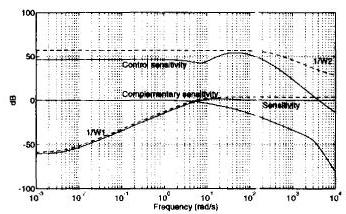
\includegraphics[max width=\textwidth]{2022_06_24_9b97a76a6ff0403ae6ddg-5}
\end{center}

Figura 6. Diseño I, valores singulares máximos

\begin{center}
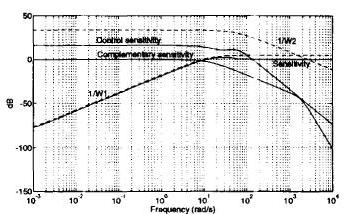
\includegraphics[max width=\textwidth]{2022_06_24_9b97a76a6ff0403ae6ddg-5(1)}
\end{center}

Figura 7. Diseño II, valores singulares máximos
\includegraphics[max width=\textwidth,]{2022_06_24_9b97a76a6ff0403ae6ddg3

Figura 8. Diseño I, respuesta de bucle cerrado con cambios de referencia
\includegraphics[max width=\textwidth,]{2022_06_24_9b97a76a6ff0403ae6ddg-6(1)}

Figura 9. Diseño I, respuesta de bucle cerrado con perturbación de velocidad
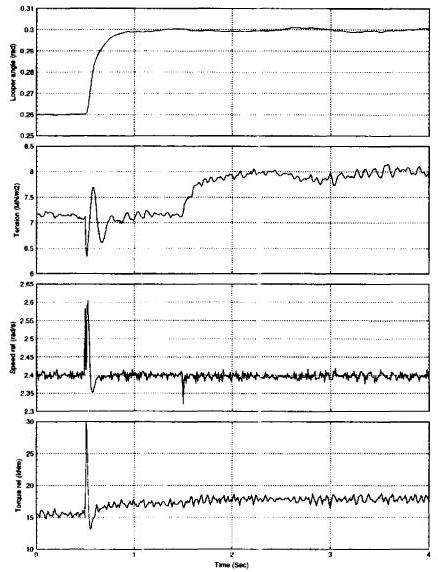
\includegraphics[max width=\textwidth,]{2022_06_24_9b97a76a6ff0403ae6ddg-6(2)}

Figura 10. Diseño II, respuesta de bucle cerrado con cambios de referencia
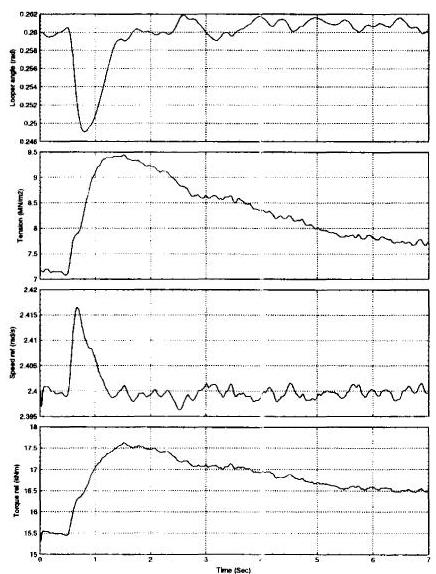
\includegraphics[max width=\textwidth,]{2022_06_24_9b97a76a6ff0403ae6ddg-6(3)}

Figura 11. Diseño II, respuesta de bucle cerrado con perturbación de velocidad


\end{document}